\section{Theorie}

Een \textbf{Brug van Wheatstone} bestaat uit twee parallel geschakelde takken,
die aangesloten worden op een spanningsbron met emk $\epsilon$ en inwendige 
weerstand $R_{i}$. Tussen beide takken legt men een brug aan met een gevoelige
stroommeter die de rol van nuldetector vervult. 
\\

Figuur 1 schets twee mogelijke opstellingen.
$R_{x}$ is de te meten weerstand, $R_{A}$ en $R_{B}$ zijn geijkte weerstanden, en R is een 
veranderlijke weerstand die men op een geijkte weerstandbank instelt. De inwendige weerstand 
van de galvanometer in de brug noemen we $R_{g}$.
\\

\begin{figure}
    \centering
    \caption{Mogelijke opstellingen bij Brug van Wheatstone}
    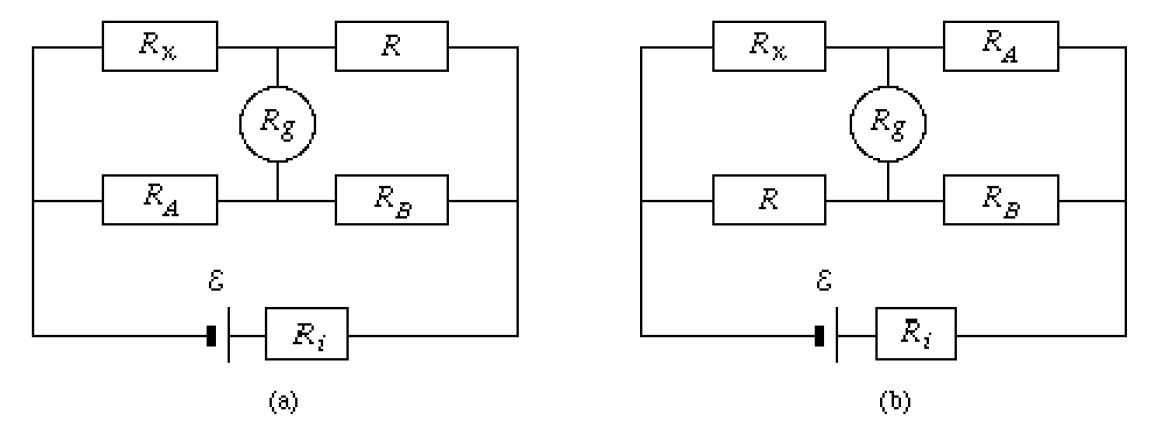
\includegraphics[width=\textwidth]{img/brug.png}
    \label{fig:grafiek}
\end{figure}

Loopt er door de galvanometer in de brug geen stroom, dat zegt men dat de stroom in evenwicht is.
In dat geval is voor schakeling $(a)$ het potentiaalverval over $R_{x}$ gelijk aan het potentiaalverval 
over $R_{A}$ en tevens is dan ook het potentiaalverval over R gelijk aan het potentiaalverval over $R_{B}$
\\

\textbf{toevoegen verwijzing naar cursus Meten en Experimenteren}